\chapter{Literature Review - Lifelong Learning \label{cha:litrev}}

In order to answer the first research question, it is important to establish a
basic understanding of the main concepts used in this work. Although,
underlying concepts can be found primarily in the domain of education, they make
a good starting point for a discussion. 

This chapter introduces the key concept of \LLLs that will be in focus
throughout the thesis. First, the origins of the term of \textit{\LLLsn} and
related concepts are discussed in Section \ref{sec:concepts}. The crucial
differences between these concepts and how they transformed over time, driven by
changing society and economics, are explored. Second, through the increasing
focus on \LLLs skills in the world of work and in higher education, Section
\ref{sec:uni} shows the need for \LLLs support in universities. Universities are
in the center of this discussion as they provide the necessary organizational
framework, theoretical principles and practical experience for \LLLs
\citep{Knapper2000}, which can be seen in the role and influence of the
universities in the educational systems of most countries as the ``keepers of
the intellectual traditions of a nation" \citep[p.~96]{Longworth2003}. Third, in
Section \ref{sec:needs} the general needs for successful \LLLs are outlined.
While no explicit requirements have been found in the literature, commonly
accepted recommendations and guidelines were discovered in various sources that
will be used as a background for further exploration in Chapter \ref{cha:model}.

\section{Literature Review Process}
The literature review on \LLLs (Chapter \ref{cha:litrev}) and a review of
institutional and open learning spaces (Chapter \ref{cha:systudy}) that provide
and support background for this thesis were conducted by systematically locating
and reviewing books, journals and conference proceedings in the area of
research. The main methods to identify relevant literature were recommendations
of domain experts and a library search. Relevant articles were identified by
reading titles and abstracts of selected journal articles and papers in
conference proceedings. Where possible the latest ten years of issues of the
following journals were looked through: ``British Journal of Educational
Technology'', ``International Journal of Lifelong Education'', ``European
Journal of Education'', ``\LLLc in Europe'', ``International Journal of Emerging
Technologies in Learning'', ``New Zealand Journal of Adult Learning'', ``Journal
of Computer Assisted Learning'', ``European Journal of Engineering Education'',
and ``International Journal of ePortfolio''. 

In addition, a keyword search was carried out on the Internet and academic
resources (such as Education Research
Complete\footnote{\url{http://www.ebscohost.com/academic/education-research-complete}},
Academic Search
Premier\footnote{\url{http://www.ebscohost.com/academic/academic-search-premier}},
Directory of Open Access Journals\footnote{\url{http://www.doaj.org}}, Google
Scholar\footnote{\url{http://scholar.google.com}}) to cover conference
publications not available in the library. The following keywords and
combinations of keywords were used in the search: ``\LLLsn'', ``life-long
learning'', ``e-learning'', ``ePortfolio'', ``e-portfolio'', ``electronic
portfolio'', ``Web 2.0'', ``learning environment'', and ``learning technology''.

This review helped to discover previous work in the area (described in Section
\ref{sec:related}), explore methods that could be applied to this research,
increase the depth and breadth of knowledge of the field, and identify domain
experts and other people working in the same field who could be valuable to
contact. Besides finding relevant information in the literature, it was also
important to identify the gaps that currently exist (more detailed discussion
can be found in Chapter \ref{cha:systudy}). It will be shown further that these
gaps are based on a lack of connection between the areas of \LLLs theories and
learning technology. While a lot of effort is put into developing theories and producing
systems that support education and learning, little substantial work exists on
combining these two areas.

As a continuous process, the literature review for this research was updated by
actively acquiring and reading the relevant articles emerging in the literature.

\section{The General Concept of \LLLc}
\label{sec:concepts}
\subsection{Terms and Definitions}

The European Commission \citeyearpar{EuropeanCommission2000} defined \LLLs as:

\longquote{All learning activity undertaken throughout life, with the aim of
improving knowledge, skills and competencies within a personal, civic, social
and/or employment-related perspective.} 

However, it is not as simple as it looks: the concept of \LLLs consists of a
variety of meanings, models and ideas. Such terms as \textit{\LLLsn},
\textit{lifelong education}, \textit{adult education}, \textit{recurrent
education}, \textit{continuing education}, and \textit{further education} create
a set of related, yet different concepts \citep{Hager2011}.

\textit{Continuing education} (also referred to as \textit{adult education}) was
introduced in the late 1970s and early 1980s. There was no common definition of
this term, but in some sources  \citep{Jarvis2004} it was described as all
learning activities which could be undertaken after compulsory schooling is
finished. Figure \ref{fig:learning} compares the main concepts in education
according to the time spent by individuals learning/studying across their
lifespan. As can be seen, continuing education was usually part-time and
occurred less frequently than other forms of education.

\begin{figure}[htb]
\centering
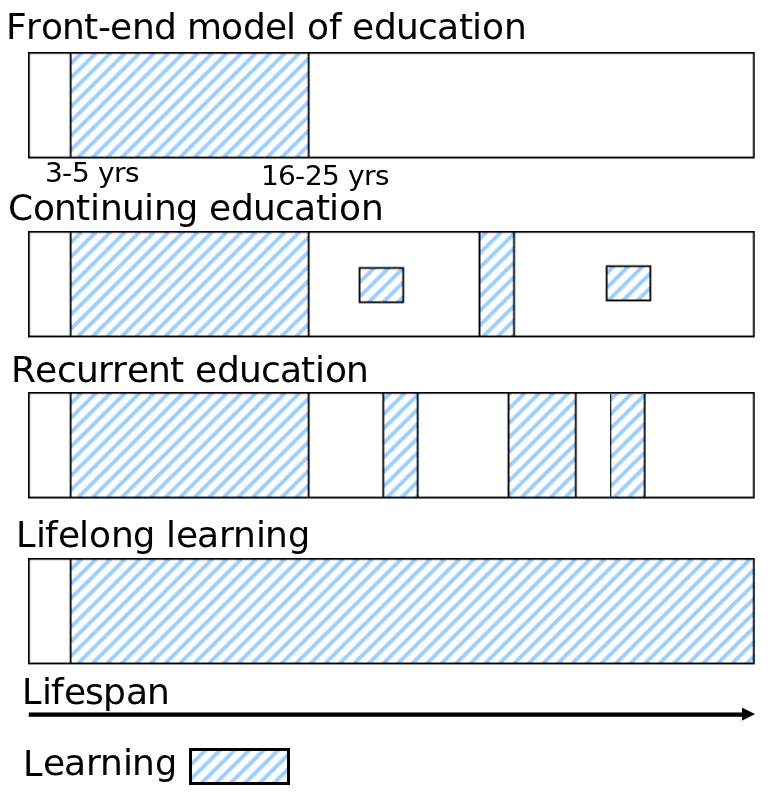
\includegraphics[width=0.57\textwidth]{CH3-F1-Learning}
\caption[Changing concepts of learning]{Changing concepts of learning 
\citep{Jarvis2004}}
\label{fig:learning}
\end{figure}

The term \textit{recurrent education} was widely used by OECD until the 1980s
\citep{Jarvis2004}. Unlike intermittent continuing education, its idea was
in allowing adults to spend full time studying in formal education sector doing
on-the-job trainings or post-compulsory education of any kind. Arguably, this
main feature of the right for full time study made the concept of recurrent
education disappear from the governments' educational agendas: it was too
expensive and difficult to support this policy.

Rejecting the concepts of recurrent and continuing education played an important
role in development of the new educational models. While they had different
underlying  philosophy, they both recognized the fact that acquisition of
knowledge should be a lifelong process, from ``cradle to grave''
\citep{Hargreaves2004}.

The origin of the term \textit{\LLLsn} goes back to the early 20th century and is
contributed to by John Dewey \citeyearpar{Dewey2004}. From his perspective,
\LLLs had to be centered on the individual's ability to take an active role in
democratic society. He saw education as a learning process which was influenced
by the growth of the individual and society, both interlinked. Dewey's key to
\LLLs was in developing active learning, enabling the individual to reflect and
change throughout life, emphasizing that non-formal education was as important
as formal education.

The concept of \textit{lifelong education} was discovered in 1972 after Edgar Faure's
Report ``Learning to Be'' for UNESCO. The concept described in this report was
announced to be the leading one for the reform in education. Faure's Report used
four principles for the lifelong education architecture \citep{Faure1972}:
vertical integration (education should occur throughout one's life); horizontal
integration (acceptance of non-formal and formal education); the democratization
of education (more widespread involvement of learners); and learning society
(restructuring of educational system). However, according to Hager's
\citeyearpar{Hager2011} analysis, UNESCO's concept of \textit{lifelong
education} puts the emphasis on formal education as the only sufficient and
relevant form of learning to provide actual \textit{education}.

\subsection{Paradigm Shift and \LLLc Today}

Almost 40 years after the idea of this lifelong education was introduced, many
governments rediscovered not lifelong education, but \LLLs \citep{Boshier2000}.
This shift was not only semantic, but also substantive, which showed that \LLLs
and lifelong education are not the same: lifelong education aimed to develop
more humane individuals and communities, while \LLLsn's goal was in retaining
and gaining new skills that would help individuals adapt to rapid changes in
their workplace \citep{Medel-Anonuevo2001}. Lifelong learning is based on the
notion of the individual learner as a consumer. And as a result if consumers
decide not to take advantage of all the opportunities they have -- then it is
their fault. Therefore, being constructed as individual activity, learning
depends entirely on personal motivation. Unlike learning, education is a
provided service \citep{Boshier2000} that requires someone to be responsible for
providing resources, developing policies, etc. The emphasis on \textit{learning}
rather than \textit{education} is significant \citep{Tuijnman2002}, as it moves
focus from the institutions onto the individual. Although, it does not mean that
institutions and governments play no role whatsoever. Their role is rather
transformed into investment in individuals and creating conditions for them to
take charge of their learning \citep{Chen2009}.

\begin{figure}[htb]
\centering 
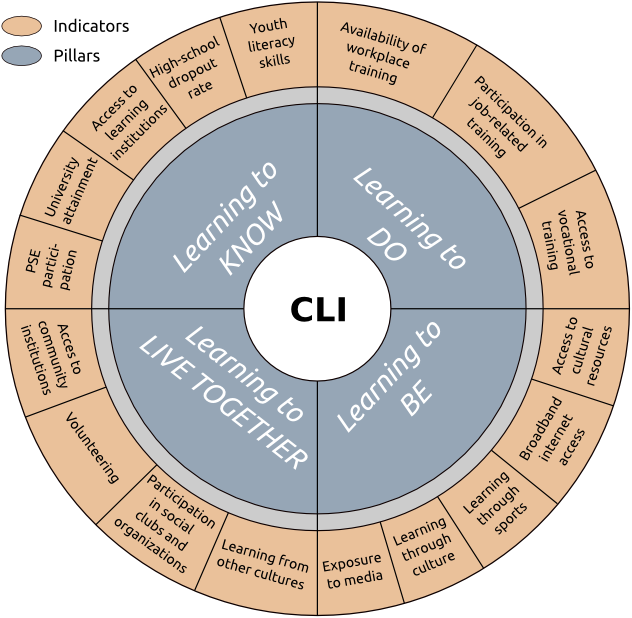
\includegraphics[width=0.8\textwidth]{CH3-F2-CLI}
\caption[The 2010 Composite Learning Index of Canada]{The 2010 Composite
Learning Index of Canada \citep{CanadianCouncilonLearning2011}}
\label{fig:cli2010}
\end{figure}

Over the last decade, lifelong learning support has become a part of official
government policy in a number of countries around the world. As an example,
European Commission established a budget of nearly 7 billion Euro for the
period of 2007-2013 for 'Lifelong learning programme' which aims to support
education and training at school, college, university, in the workplace and in
the community across Europe \citep{TheEducation2009}. In New Zealand a number of
governmental documents \citep{NewZealandMinistryofEducation2008} now mention
the ``success of all New Zealanders through lifelong learning". As a result, the
national tertiary education system of the country has been transformed to
support lifelong learning ideals \citep{Benseman2006}.

In 2006, the Canadian Council on Learning developed the 17 indicators and 26
specific measures (Figure \ref{fig:cli2010}) called Composite Learning Index
(CLI) that are used to calculate annual progress in \LLLs in the country
\citep{CanadianCouncilonLearning2011}. Using CLI, Canadian government expects to
draw attention to the benefits of \LLLs and demonstrate learning opportunities
that occur outside of classroom settings. In August 2010 the European Union
adopted this Index as European \LLLc Indicators (ELLI). Similar to CLI, ELLI
were using UNESCO approach of four pillars of learning: Learning to Know,
Learning to Do, Learning to Be, and Learning to Live Together
\citep{ELLIDevelopmentTeam2010}.

\subsection{Components and Attributes of Lifelong Learning}
In terms of purposeful learning activities \LLLs consists of the following
components \citep{Longworth2003, Tuijnman2002}:

\begin{itemize}
  \item Formal learning -- institutionally graded, and hierarchically structured
system, often leads to qualification;
  \item Non-formal learning -- organized systematic educational activity
  external to formal education;
  \item Informal learning -- planned or not planned, but conscious learning from
the experience;
  \item Incidental learning -- not intentional, an accompaniment to everyday
  life, learning during the action.
\end{itemize} 

\begin{figure}[htb]
\centering
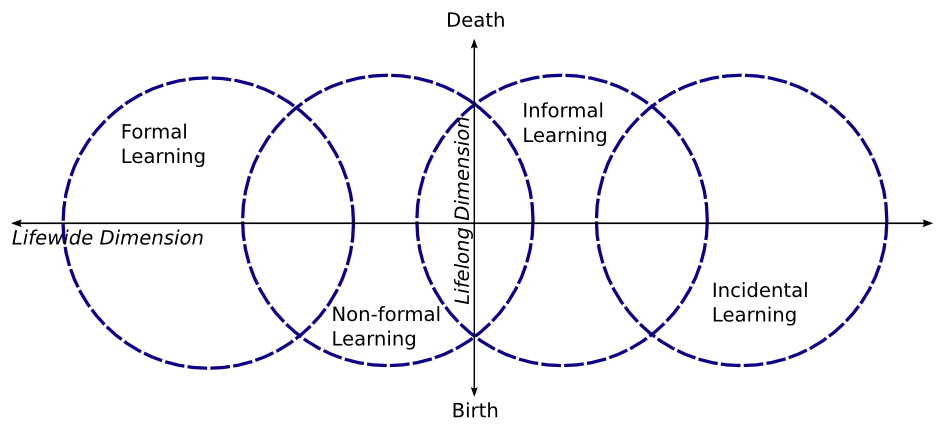
\includegraphics[width=0.8\textwidth]{CH3-F3-LLLFramework}
\caption[Framework for \LLLc]{Framework for \LLLc (based on
\citealp[p.~11]{Divjak2004})}
\label{fig:lllfmwrk}
\end{figure}

Some researchers \citep{Longworth2003} recognize only two categories of lifelong
learning, formal and non-formal, leaving informal and incidental parts of it as
the elements of non-formal learning. Boshier \citeyearpar{Boshier2000} states
that the current reality is such that the formal and non-formal categories of
\LLLs are like ``two parallel railway lines. Both cross the landscape but never
touch'' (p. 11), explaining this way that formal setting have practically
nothing to do with non-formal. 

From another perspective, \LLLs encompasses the elements of self-direction,
long-term and life-wide learning \citep{Schuetze2006}. Rubenson
\citeyearpar{Rubenson2002} called these \textit{three fundamental attributes of \LLLs}:

\begin{itemize}
  \item Lifelong -- means everything from cradle to grave;
  \item Life-wide -- takes place outside the formal education system;
  \item Self-directed -- is guided by the learners themselves and does not
  limit itself to education.
\end{itemize} 

Weert and Kendall \citeyearpar{Kendall2004} gathered other essential
characteristics of \LLLsn:

\begin{itemize}
  \item Most of \LLLs occurs outside of the classroom and is not triggered by
  textbooks;
  \item The driving force in \LLLs is self-motivation and active participation
  of learners;
  \item Lifelong learning involves interactions, groups, community learning and
  other social activities;
  \item Solving artificial tasks does not matter in \LLLsn. Achievements in
  real-life situations, measured by common standards, are important;
  \item Lifelong learning is learner-centred and aims for personal
  achievements;
  \item Lifelong learners should maintain an achievements portfolio.
\end{itemize} 

These characteristics describe \LLLs as demand-driven, flexible, social and
personal at the same time. 

Over recent years the skills that provide \LLLs ability were identified. They
include: solving problems, critical thinking, utilizing technology, and
information literacy; working with others in teams, communication skills,
leadership and social interaction skills; self-management; collecting, analyzing
and organizing information; planning and organizing activities; cultural
awareness and understanding
\citep{Brooks2008,Heinrich2007,Otala1997,Pitman2009}. 

\begin{figure}[htb]
\centering
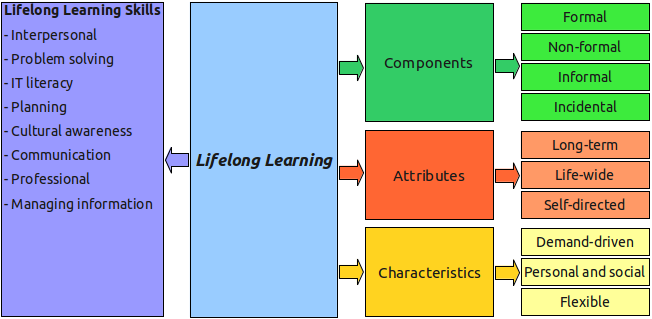
\includegraphics[width=1\textwidth]{CH3-F4-LLLDimension}
\caption{\LLLc Dimensions}
\label{fig:llldim}
\end{figure}

Figure \ref{fig:llldim} summarizes all concepts mentioned in this section.
Hereinafter, any further reference to \LLLs will be made in terms of these
concepts.

\section[\LLLc in Universities]{\LLLc in Universities\footnote{This section was
adopted from the section originally published as part of Chapter 8 ``The Role of
Institutions in Creating Student-Focused Virtual Learning Spaces with ePortfolio
Systems'' of the book ``Physical and Virtual Learning Spaces in Higher
Education: Concepts for the Modern Learning Environment". Full reference can be
found in Publications section.} }

\label{sec:uni}

As \LLLs includes the concepts of \textit{life-long}, \textit{self-directed}
and \textit{life-wide} learning, it has following significant implications. As
already mentioned above, \textit{life-long} means the full life span of an
individual. From the institutional view, it starts when students are enrolled in
the university and finishes when they graduate. \textit{Self-directed} learning
in academic environment is based on being an active, highly-motivated student
acquiring and enhancing new skills and knowledge. The \textit{life-wide}
component of learning implies that learning can and should not occur only
through formal university study, as personal and professional development takes
place in many contexts. Attwell \citeyearpar{Attwell2007} considers the fact
that everyday non-formal types of learning are not connected to institutional
formal education to be the major issue of modern learning, which can make
students see their study at university as ``something irrelevant to their
identities'' (p. 4). For successful \LLLsn, progress of the achievements should
be recorded and maintained over a long period and across various sources, formal
as well as non-formal \citep{Kay2008}.

%%A \LLLs environment needs to acknowledge this and allow
%%learners to record and reflect on experiences from all these contexts.

The importance of \LLLs skills in addition to academic and subject knowledge has
been increasingly emphasized in the workplace and public policy
\citep{Morgan-Klein2007,Sutherland2006}. Individuals today need to continue to
update and upgrade their skills and knowledge even after completing formal
education in order to survive in the changing world. Otala
\citeyearpar{Otala1997} states that required flexibility and adaptability to
these rapid changes are gained through ``better developed learning skills and
the right attitudes that help individuals quickly and easily learn new things''
(p. 456). Therefore, current students need to ``possess something more than
skills which grow obsolete as technology advances'' \cite[p.~195]{Field2003}. 

Higher education institutions have responded to the need for \LLLs skills by
defining their own strategies to promote \LLLsn. Many institutions in Europe,
the United States, Australia and New Zealand now explicitly express the \LLLs
characteristics they strive for in their graduates \citep{Scanlon2006}.
Australian universities, such as Curtin University, have made policy
declarations committing to graduate attributes across their programmes
\citep{CurtinUniversity2006}. The College of Sciences of Massey University has
formulated a draft \LLLs policy \citep{MasseyUniversity2008} that expresses
values, support and expectations in regards to \LLLsn. Graduate profiles, naming
\LLLs skills such as critical thinking, effective communication, teamwork and
leadership have been established for many degree programme
\citep{Davies2003,McAlister2003}. The accreditation criteria for engineering
degrees now refer to and demand soft skills \citep{Aller2005,Muffo2001}. The
need for a holistic education and the development of students beyond technical
competency is requested
\citep{Brakke2002,Davies2003,Dowling2006,Fallows2003,Grabowski2004,Hernon2006}.

In order to enact policy academics need to incorporate development opportunities
for these skills into their teaching and learning designs. While individual
academics succeed in doing so by using techniques such as group work, reflective
journals and authentic assessment \citep{Clarke2003,Lombardi2008}, universities
are far from achieving the required levels of \LLLs skills in their graduates.

The possible explanation of this might be that while graduate profiles express
graduate attributes and \LLLs skills, the individual courses making up the
degrees have not been adjusted accordingly \citep{Hughes2010}. One consequence
of this is that students are not presented with a coherent picture across their
courses and that it is too easy to disregard the messages given in single
courses. Some academics may lack awareness, skills and support to fully
incorporate the development of \LLLs skills into their teaching. Academics who
do not consciously practice their own \LLLs skills development will find it
difficult to lead and to inspire their students \citep{Linden2003}. Yet,
students need guidance in developing \LLLs skills \citep{Leone2019}, both to
recognise their importance and to acquire knowledge on \textit{how to} study
\citep{Medel-Anonuevo2001}. The currently dominant academic systems are in
conflict with the characteristics of \LLLs skills. Instead of supporting the
needs of learning to be self-directed, life-wide and lifelong, these systems are
assessment-driven and focus on course content and duration.

\section{Requirements for Successful \LLLc}
\label{sec:needs}
Based on considerations outlined earlier in this chapter, this section brings
together the requirements for provision of successful \LLLs support for
students. While no explicit set of requirements has been found, the
literature identifies a number of guidelines and recommendations that have to be
satisfied in order to achieve successful \LLLs support in universities:
 
\begin{itemize}
  \item Universities should provide support for all aspects of \LLLs (formal,
  informal, non-formal, incidental) \citep{Smidt2011};
  \item Students need guidance on various levels \citep{Leone2019};
  \item Lecturers should be an active facilitators and promote involving
  learning experiences \citep{Leone2019}; 
  \item Learning materials should be organized in the way that would help
students learn how they learn \citep{Medel-Anonuevo2001};
  \item Communication and collaboration are essential parts of learning process
  \citep{Schaffert2008};
  \item Learning progress should be recorded from various sources and maintained
  over a long period of time \citep{Kay2008};
  \item Students need to be aware of their personal achievements
\citep{Schuetze2006};
  \item Students should develop understanding and confidence in their knowledge
  and be able to address higher-order skills (graduate attributes in university
  context) \citep{Hart1999};
  \item Students should be able to evaluate and reflect on their own performance
and learning progress \citep{Mourtos2003}.
\end{itemize} 

These theoretical recommendations will be used to guide further exploration of
 how \LLLs can be supported using technical solutions available in universities.

\section{Summary} 

Following from the discussions in this chapter, it is important to emphasize
the following key points: \LLLs plays an important role in current global
economics and society; \LLLs skills have become a fundamental part of personal
development; governments and educational institutions, universities in
particular, are attempting to promote and support \LLLsn; at this stage, \LLLs
support currently provided in universities is not sufficient to satisfy the
needs of students as lifelong learners.

In order to support this argument, the next chapter will review the world of
learning spaces that are currently used in universities and outside of
educational sector to support various learning activities. The connection and
gap that exists between these systems from the \LLLs perspective will be
thoroughly explored.
